\chapter{DES}

\section{Introduzione Data Encryption Standard (DES)}
Primo protocollo a chiave segreta o simmetrico, utilizzato per molto tempo. Ci spiega abbastanza chiaramente quali sono le caratteristiche di un cifrario a chiave segreta (funzioni matematiche che prendono un messaggio, ci mischiano una chiave segreta condivisa col destinatario e tirano fuori il crittogramma. Il destinatario riceve il crittogramma e con la stessa chiave segreta esegue l'operazione inversa). Ci sono due criteri fondamentali alla base di questo tipo di cifrari:
\begin{itemize}
	\item diffusione : alterazione del testo in chiaro, significa "spargere" i caratteri (del messaggio e della chiave) su tutto il testo cifrato;
	\item confusione : combinazione in modo complesso del messaggio e della chiave, per non permettere al crittoanalista di separare queste due sequenze mediante un'analisi del crittogramma (impastiamo uniformemente messaggio e chiave, possibile se ho tanta randomness).
\end{itemize}
Bisogna considerare che ci stiamo muovendo in un campo empirico, non ci sono teoremi, tutte le cose che facciamo durante questa parte del corso sono basate sulla pratica (es: un sistema è sicuro se non è ancora stato violato). L’esempio classico di cifrario simmetrico con diffusione e confusione è il Data Encryption Standard, brevemente
DES, introdotto dalla IBM nel 1977 e divenuto per ben oltre vent’anni lo standard per le comunicazioni commerciali riservate ma "non classificate". I criteri di diffusione e confusione vengono soddisfatti attraverso una serie di messaggi sulla chiave, si tratta di permutazione, espansione (di bit) e compressione. Analizzeremo tutto il flusso di informazioni elaborate dal DES facendo riferimento all' S-box (unica parte non lineare del procedimento), da cui dipende fortemente la sicurezza del cifrario (una piccola modifica all'S-box può portare danni enormi). L'implementazione del DES è pubblica, da 50 anni, si parte dal concetto che la robustezza del cifrario non dipende dal fatto che viene tenuto nascosto, bensì dal fatto che non c'è una chiave condivisa. Il nuovo cifrario, che lo sta sostituendo è l'AES (filosoficamente simile al DES).

\section{Struttura}

Abbiamo un messaggio di n bit, divisi in blocchi di 64 bit, ogni blocco è cifrato in maniera indipendente dagli altri (questo ci permette di sfruttare il parallelismo, codifichiamo in parallelo, basta avere più processori). Il DES procede per fasi, ci sono 16 round in cui si ripetono le stesse operazioni, l'output generato da un round $x_{i-1}$ farà da input al round $x_i$.
\subsection{La chiave segreta}

La chiave $k$ è composta da 64 bit (8 byte), però ne vengono usati sono 56 come chiave, perchè 8 di questi 64 vengono utilizzati come bit di parità (rudimentale metodo di correzione d'errore, funziona se ho un numero di 1 pari). Dalla chiave $k$ vengono create $r$ sottochiavi ($r$ = 16):\\
$k[0], k[1], ..., k[r-1]$ impiegate una per fase.
Il messaggio viene diviso in due metà S e D (sinistra e destra). In ciascuna fase si eseguono le due operazioni: $D \rightarrow S$ e $f(k[i - 1], D, S) \rightarrow D$, dove $f$ è una opportuna funzione non lineare e $i = 1, ..., r$. Alla fine delle $r$ fasi le due metà vengono nuovamente scambiate e poi concatenate per produrre il crittogramma
finale.

\begin{figure}[htp]
	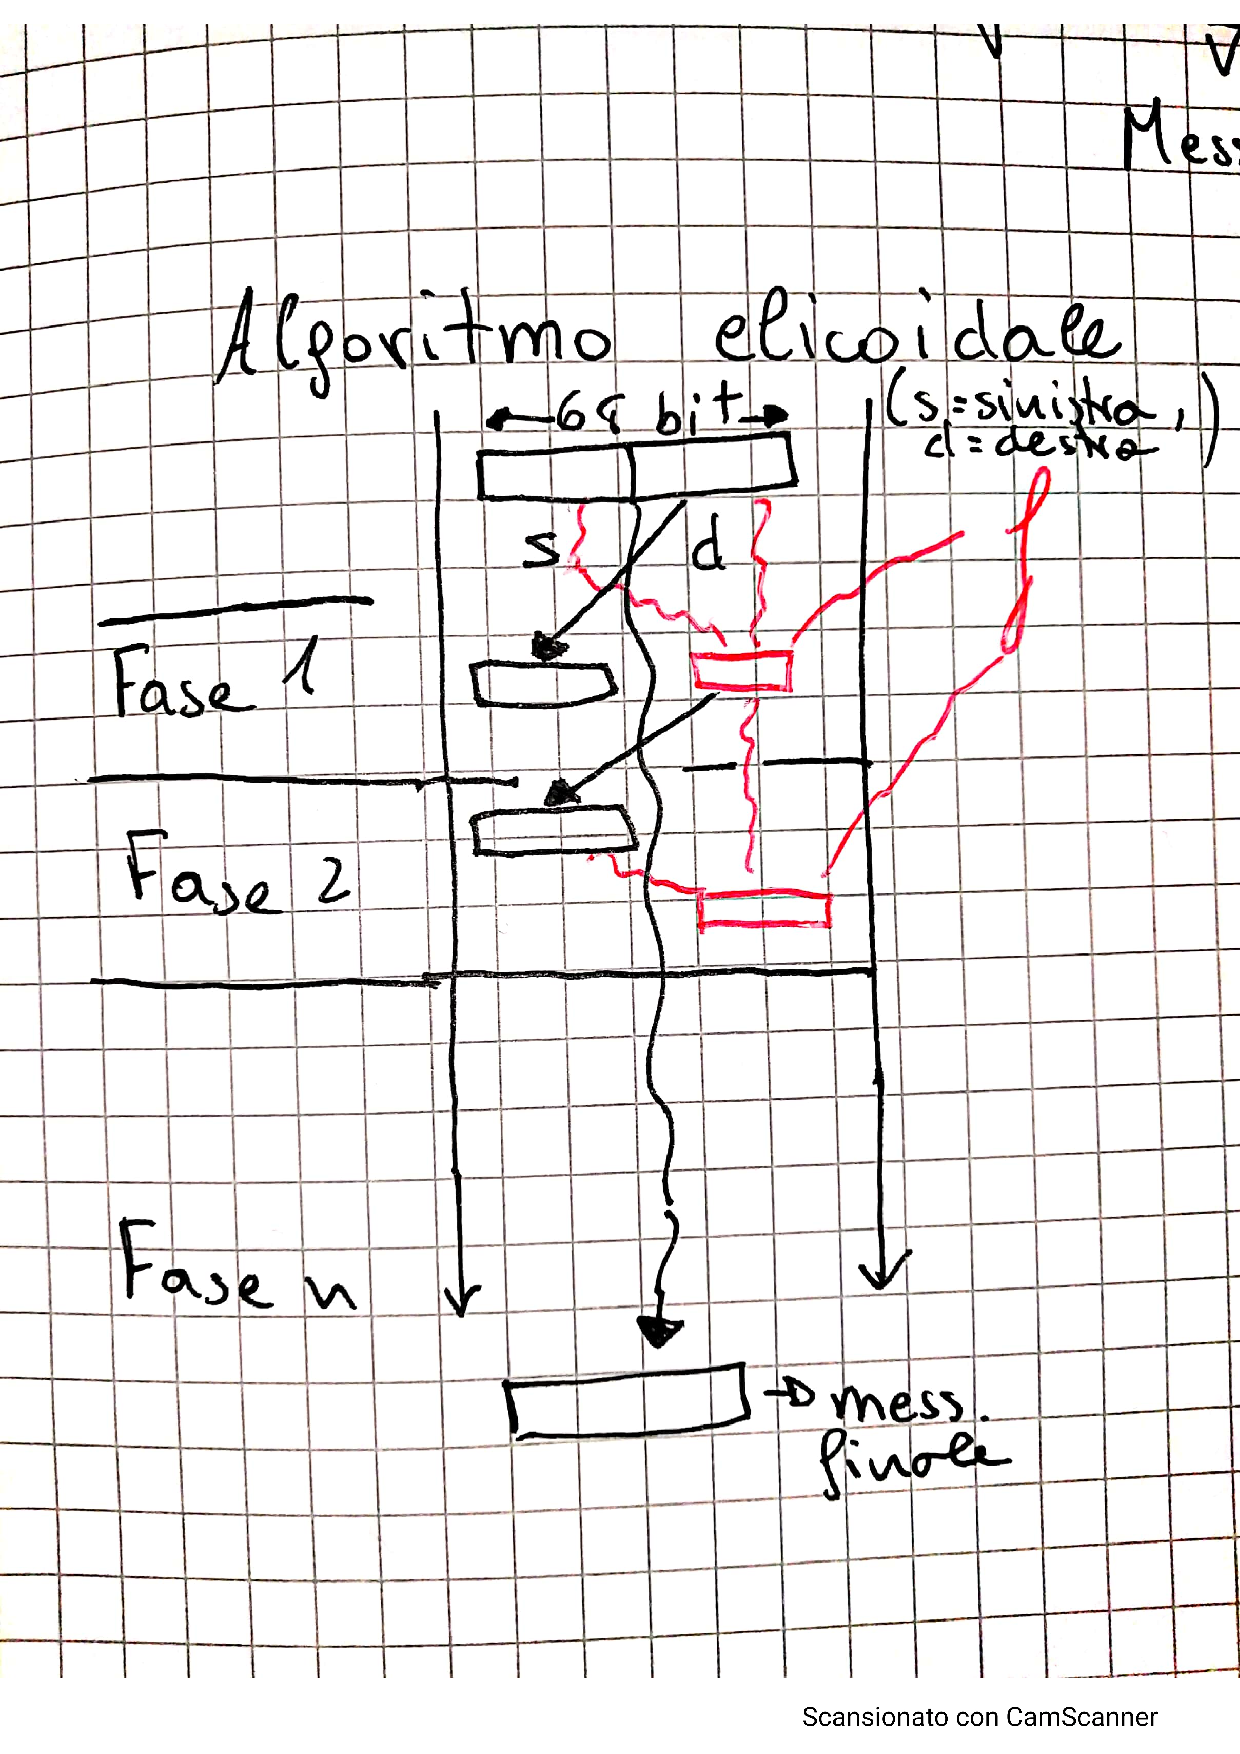
\includegraphics[width=\linewidth]{./img/algoritmo_elicoidale.pdf}
	\label{img:algoritmo_elicoidale}
\end{figure}


\subsection{Primo colpo di genio (il genio non esiste... e a volte è un idiota)}
La cosa molto sorprendente è che la decifrazione (decodifica del crittogramma) consiste nel prendere il crittogramma, riapplicargli l'algoritmo con le chiavi invertite (la sequenza delle r sottochiavi viene ribaltata). Questo non è assolutamente banale.

\section{Funzionamento}

Lo schema appena descritto si realizza usando:
\begin{itemize}
	\item permutazioni di bit (disposizioni con $n = k$);
	\item espansioni (ho una sequenza di bit lunga $n$ e la voglio trasformare in una nuova sequenza lunga $n + i$, sto di fatto espandendo la sequenza iniziale);
	\item compressioni di sequenze binarie (operazione inversa rispetto all'espansione, ho un tot di bit e ne voglio di meno, ci saranno bit inutilizzati);
	\item alcune semplici funzioni combinatorie tra messaggio e chiave.
\end{itemize}
 L’insieme di queste operazioni garantisce che alla fine del processo ogni bit del crittogramma dipenda da tutti i bit della chiave e da tutti i bit del messaggio in chiaro, rispondendo così ai criteri di confusione e diffusione proposti da Shannon.
 L’estensione della chiave con i bit di parità garantisce la corretta acquisizione e memorizzazione di tutti i bit della chiave stessa, condizioni cruciali per la decifrazione dell’intero crittogramma. La stessa protezione non è richiesta per il messaggio poiché un errore locale in esso si propaga nel crittogramma, ma è poi riprodotto identico all’originale nel messaggio decifrato con danno in genere
irrilevante per la trasmissione.L’estensione della chiave con i bit di parità garantisce la corretta acquisizione e memorizzazione di tutti i bit della chiave stessa, condizioni cruciali per la decifrazione dell’intero crittogramma. La stessa protezione non è richiesta per il messaggio poiché un errore locale in esso si propaga nel crittogramma, ma è poi riprodotto identico all’originale nel messaggio decifrato con danno in genere
 irrilevante per la trasmissione. L'estensione ci permette di aggiungere un grado di certezza riguardo il fatto che stiamo utilizzando la chiave corretta, perchè se ci sono errori singoli sulla chiave viene identificato l'errore ed è molto utile, perchè anche un bit sbagliato nella chiave può portare ad uno stravolgimento del crittogramma (ma è anche vero che, se il ricevitore si accorge dell'errore può richiedere la ritrasmissione dell'informazione, questo perchè il canale su cui si spedisce è protetto dalla codifica; mentre attenzione, il canale in cui viene spedita la chiave è costoso, dunque sulla chiave errori non ne vogliamo fare). \\
 Nota importante : fra hardware è molto raro che ci sia un errore, per questo si sfrutta il bit di parità, che lavora bene solo su un numero dispari di errori.
 \subsection{Rappresentazione grafica}
 Guida:
 \begin{itemize}
 	\item la chiave $k$ parte a 64 bit ma attraverso il processo T (trasposizione), il quale elimina i bit di parità, diventa 56 bit;
 	\item il messaggio passa attraverso PI = "permutazione iniziale", in poche parole mischia le carte (scambiano di posto i bit);
 	\item All'uscita viene effettuata una ulteriore permutazione, PF è il contrario della permutazione iniziale (lo schema in alto a destra ne spiega il funzionamento);
 \end{itemize}

\begin{figure}[htp]
	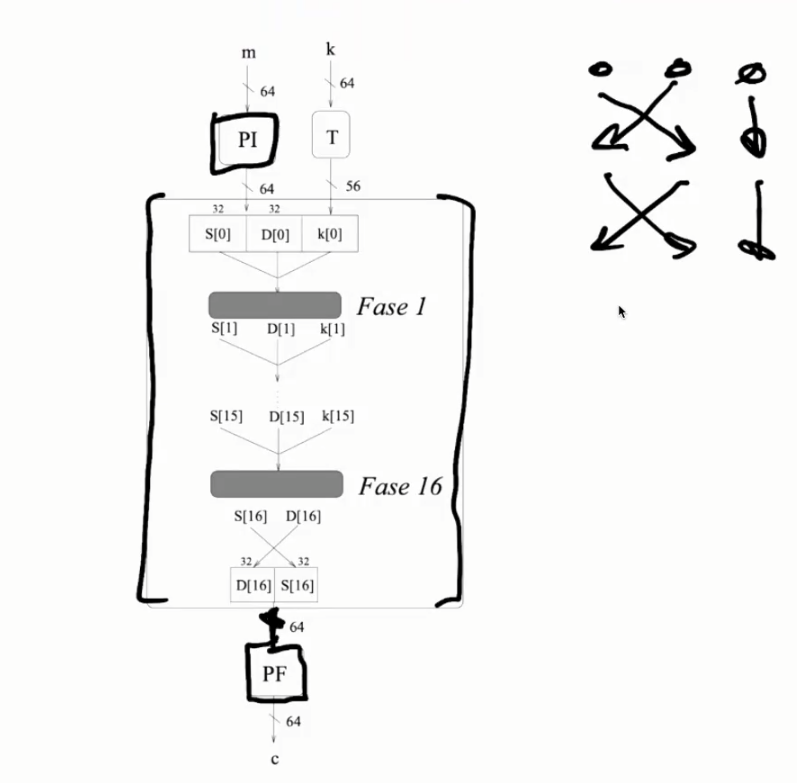
\includegraphics[width=\linewidth]{./img/DES.png}
	\label{img:DES}
\end{figure}

\subsubsection{Analisi processi}

\begin{figure}[htp]
	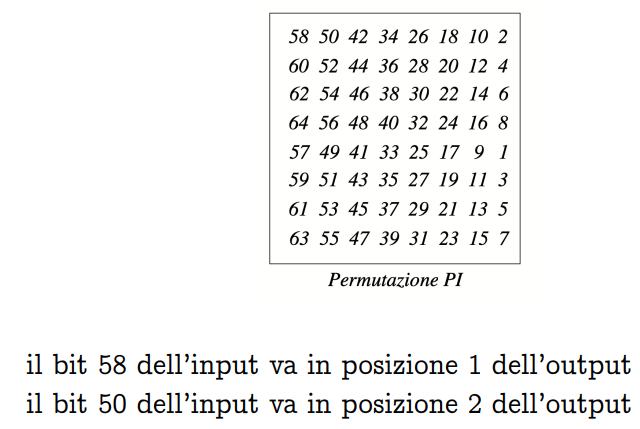
\includegraphics[width=250pt]{./img/DES_permutazionePI.png}
	\caption{Permutazione PI}
	\label{img:DES_permutazionePI}
\end{figure}

\begin{figure}[htp]
	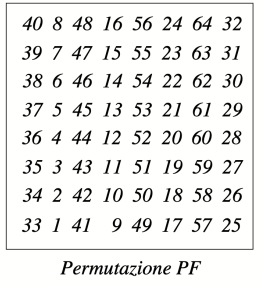
\includegraphics[width=150pt]{./img/DES_permutazionePF.png}
	\caption{Permutazione PF}
	\label{img:DES_permutazionePF}
\end{figure}

\begin{figure}[htp]
	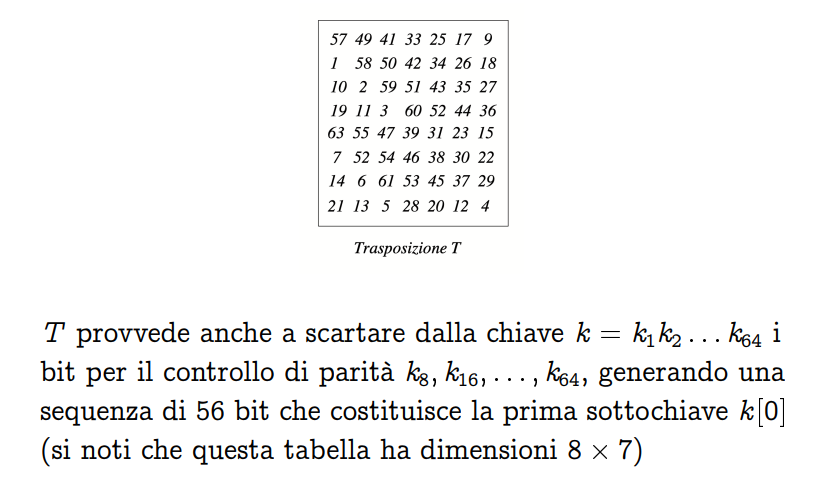
\includegraphics[width=300pt]{./img/DES_trasposizione.png}
	\caption{Trasposizione T}
	\label{img:DES_trasposizione}
\end{figure}


Nella trasposizione è interessante notare che i bit 8, 16, ..., 56 sono stati rimossi, perchè saranno i bit di parità, questo trasformerà la dimensione della tabella, in 8x7.

\section{DES : fase i-esima}

La fase i-esima prende in input 32 bit, che provengono dalla fase precedente e la chiave i-esima della fase precedente (i 56 bit provenienti dalla trasposizione). Distinguo due colonne:
\begin{itemize}
	\item colonna di sinistra
	\begin{itemize}
		\item viene svolto l'incrocio, mostrato nella immagine "algoritmo elicoidale";
		\item i 32 bit della fase i-1 di destra formano i 32 bit della fase i della parte sinistra;
		\item in parallelo il messaggio di destra della fase i-1 entra in EP, che fa una espansione, portando il messaggio a 48 bit. Il messaggio di 48 bit verrà poi messo in xor con CT;
		\item terminato lo xor il messaggio entra in S, ritornando ad essere di 32 bit;
		\item infine il messaggio passa in P (permutazione) e si mette in xor con il messaggio di sinistra della fase i - 1, formando così il messaggio di destra della fase i.
	\end{itemize}
	\item colonna di destra
	\begin{itemize}
		\item c'è una fase di calcolo e poi il risultato viene passato alla colonna di sinistra;
		\item viene inoltre generata la chiave della fase successiva;
		\item i 28 bit di SC entrano dentro CT, inoltre vengono ricongiunti per formare la chiave del passo i-esimo.
	\end{itemize}
\end{itemize}

\begin{figure}[htp]
	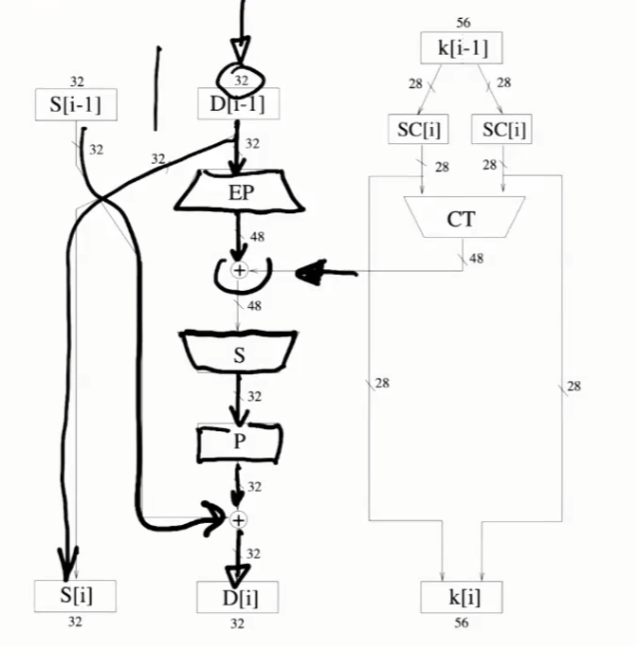
\includegraphics[width=300pt]{./img/fase_i_esima_des.png}
	\caption{Qui viene mostrato un arbitrario passaggio intermedio, successivamente nel capitolo verranno mostrati analiticamente tutti i passaggi}
	\label{img:fase_i_esima_des}
\end{figure}

\newpage

\section{SC - shift ciclici}

Si tratta dello shift bit a bit, può avvenire sia a destra che a sinistra, è diverso da quello tradizionale perchè shifta sfruttando un criterio diverso. La sottochiave $k[i - 1]$ di 56 bit, ricevuta dalla fase precedente, viene suddivisa in due metà di 28 bit
ciascuna. Su ognuna di queste la funzione $SC[i]$ esegue uno shift ciclico verso sinistra di un numero di posizioni definito come segue: $SC[i] = 1$ per $i = 1, 2, 9, 16,$
$SC[i] = 2$ altrimenti (per i fini del corso non è così importante capire il perchè). Le due parti così traslate vengono concatenate in un unico blocco di 56 bit che costituisce la sottochiave $k[i]$ per la fase successiva, ma... servono anche come chiavi dopo l'esecuzione di CT.

\begin{figure}[htp]
	\centering
	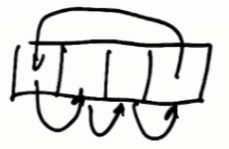
\includegraphics[width=100pt]{./img/shift_a_destra.png}
	\caption{Esempio di shift ciclico a destra}
	\label{img:shift_a_destra}
\end{figure}

\section{La permutazione con selezione di CT}

CT prende in input due segmenti da 28 bit. La combinazione delle funzioni SC[i] e CT garantisce che in ogni fase venga estratto dalla sottochiave un diverso
sottoinsieme di bit per la cifratura. Si calcola che nella cifratura ogni bit della chiave originale k partecipi in media a 14 fasi (vuol dire che se ho 56 bit, ognuno di essi fruisce nella cifratura, questo implementa il concetto di diffusione, tutto ciò che ho in input viene diffuso nell'algoritmo di cifrazione). Selezione perchè alcuni bit vengono buttati via e gli altri rimanenti vengono permutati, infatti si passa da 56 a 48 elementi. 

\section{EP - estensione e permutazione}

Entrano 32 bit e ne devono uscire 48. Abbiamo che 16 bit di ingresso vengono duplicati, per esempio il bit 32 è copiato nelle posizioni 1 e 17 dell'uscita. 

\section{S}

Secondo molti è la parte cruciale di questo algoritmo, in quanto garantisce la sicurezza che lo contraddistingue. Da 48 bit si torna a 32, i 48 bit si dividono in gruppi da 6, vengono dunque formati 8 gruppi totali. Ogni gruppo fa uscire 4 elementi, da questo si arriva a 32 bit. I gruppi sono le uniche parti non lineari di DES. Come si fanno a descrivere questi gruppi? Le riscriviamo con la tabella sottostante, abbiamo 16 colonne, ciò significa che per indicizzare la colonna da 0 a 15 occorrono 4 bit, per indicizzare le righe da 0 a 4 ne occorrono 2. 2 + 4 = 6 bit, che sono esattamente il numero di ingressi dei gruppi. La funzione S-box costituisce la parte magica di DES, su cui si basa la sicurezza del cifrario. Questa funzione, progettata con molta cura dalla IBM e modificata con altrettanta cura dalla NSA, costituisce la
parte cruciale e "magica" su cui si basa la sicurezza del cifrario. Essa consta di otto sottofunzioni combinatorie $S_1, S_2, ..., S_8$. L’ingresso di 48 bit viene decomposto in otto blocchi $B_1, B_2, ..., B_8$ di 6 bit ciascuno che costituiscono l’ingresso alle sottofunzioni di pari indice.
Sia $B_j = b_1b_2b_3b_4b_5b_6$. Questi bit vengono divisi in due
gruppi $b_1b_6$  e  $b_2b_3b_4b_5$ che definiscono due numeri $x, y$,
con $0 \leq x \leq 3 $ e $0 \leq y \leq 15$, utilizzati per accedere alla
cella di riga x e colonna y in una tabella che definisce la
sottofunzione $S_j$. Il numero ivi contenuto è compreso tra 0
e 15, ed è quindi rappresentato con 4 bit che costituiscono
l’uscita di $S_j$ realizzando una compressione da 6 a 4 bit. Complessivamente gli otto blocchi generano una sequenza
di 32 bit. I blocchi EP e S sono studiati in modo che
tutti i bit di $D[i - 1]$ influenzino l’uscita di $S$ (significa che se io cambio un bit da 0 ad 1 o viceversa in $D[i]$, questo influisce sul risultato della combinazione di EP con S), senza di
che non sarebbe poi possibile decifrare il messaggio.

\section{P}

P è una permutazione di 32 bit che genera il blocco finale $D[i]$.

\section{Linearità e non linearità}

Tutte le funzioni applicate dal cifrario, a eccezione della
S-box, sono lineari se riferite alla operazione di XOR,
cioè vale $f(x) XOR f (y)$ = $f (x XOR y)$ ove $f$ è una funzione
permutazione, espansione o compressione di un vettore
binario e $x, y$ sono vettori binari arbirari. Ciò invece non
si verifica se $f$ è una delle otto funzioni della S-box che
sono dunque non lineari. Si stima che questo contribuisca
in modo determinante alla sicurezza del cifrario. E' più facile predire un comportamento lineare rispetto ad un comportamento non lineare. Una funzione è lineare se è chiusa rispetto a somma e prodotto.

\section{Attacchi}

Purtroppo le chiavi possibili per il DES, ai giorni nostri, essendo formate da 56 bit sono fattibili da violare, i computer che abbiamo ad essere non è un problema elaborare $2^{56}$ combinazioni. Ci sono inoltre proprietà che ci permettono di dimezzare il numero di chiavi. A fronte di questa particolarità il DES è diventato sempre meno sicuro, dunque si è deciso di aumentare il numero di bit legati alle chiavi. Il punto debole del DES è costituito dal fatto che la chiave sia composta da 56 bit, questo significa che il protocollo è piccolo. Attenzione però, se arrivo a dover scandire tutte le $2^{56}$ chiavi significa che il protocollo non è stato violato, per essere violato occorre decifrare il crittogramma senza utilizzare tutte le chiavi.